\newcommand\toplisting[0]{\hrule\vspace{5pt}}
\newcommand\bottomlisting[0]{\vspace{4pt}\hrule}

\newcommand\customlisting[4]{
  \begin{figure}[ht]
    \centering
    \begin{minipage}{#2\linewidth}
      \toplisting
      \lstset{caption=#3,label=#1}
      \input{#4}
      \bottomlisting
    \end{minipage}
  \end{figure}
}

\newcommand\transportInterface[1]{
  \begin{figure}[ht]
    \centering
    \begin{minipage}{0.8\linewidth}
      \toplisting
      \input{transport/transport/core/src/main/scala/transport/Transport.listings}
      \lstset{caption=#1,label=transportInterface}
      \input{transport/transport/core/src/main/scala/transport/package.listings}
      \bottomlisting
    \end{minipage}
  \end{figure}
}

\newcommand\actorWrapper[1]{
  \customlisting{actorWrapper}{0.92}{#1}
    {transport/examples/report-listings/jvm/src/main/scala/examples/ActorWrapper.listings}
}

\newcommand\yellingActor[1]{
  \customlisting{yellingActor}{0.68}{#1}
    {transport/examples/report-listings/jvm/src/main/scala/examples/YellingActor.listings}
}

\newcommand\rpcExample[1]{
  \begin{figure}[ht]
    \centering
    \begin{minipage}{0.74\linewidth}
      \toplisting
      \input{transport/examples/report-listings/jvm/src/main/scala/examples/RpcExampleApi.listings}
      \vspace{12pt}
      \input{transport/examples/report-listings/jvm/src/main/scala/examples/RpcExampleServer.listings}
      \vspace{12pt}
      \lstset{caption=#1,label=rpcExample}
      \input{transport/examples/report-listings/jvm/src/main/scala/examples/RpcExampleClient.listings}
      \bottomlisting
    \end{minipage}
  \end{figure}
}

\newcommand\engineInterface[1]{
  \customlisting{engineInterface}{0.75}{#1}
    {survivor/lag-comp/src/main/scala/AbstractEngine.listings}
}

\newcommand\stateGraph[1]{
  \begin{figure}[ht]
    \centering
    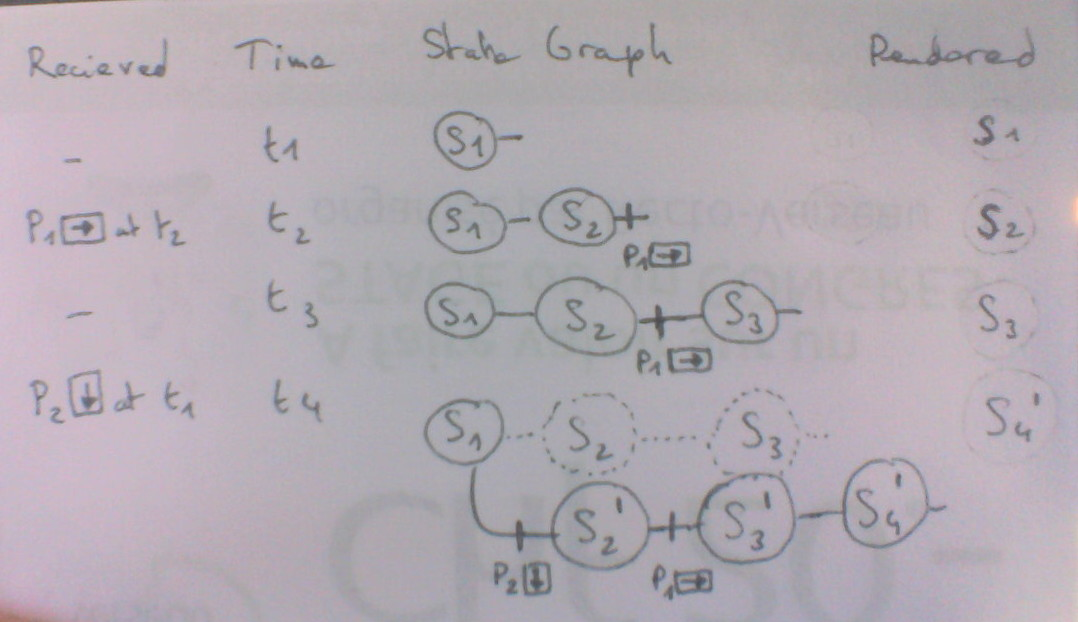
\includegraphics[width=0.8\textwidth]{state-graph}

      % \usepackage[usenames,dvipsnames]{pstricks}
% \usepackage{epsfig}
% \usepackage{pst-grad} % For gradients
% \usepackage{pst-plot} % For axes
% User Packages:
% 
% 
\psscalebox{1.0 1.0} % Change this value to rescale the drawing.
{
\begin{pspicture}(0,-1.2225)(6.0,1.2225)
\pscircle[linecolor=black, linewidth=0.03, dimen=outer](0.4,0.8225){0.4}
\rput(0.4,0.8225){\emph{S\textsubscript{1}}}
\pscircle[linecolor=black, linewidth=0.03, dimen=outer](5.2,-0.3775){0.4}
\rput(5.2,-0.3775){\emph{S'\textsubscript{4}}}
\pscircle[linecolor=black, linewidth=0.03, dimen=outer](2.0,-0.3775){0.4}
\rput(2.0,-0.3775){\emph{S'\textsubscript{2}}}
\pscircle[linecolor=black, linewidth=0.03, dimen=outer](3.6,-0.3775){0.4}
\rput(3.6,-0.3775){\emph{S'\textsubscript{3}}}
\pscircle[linecolor=black, linewidth=0.03, linestyle=dashed, dash=0.17638889cm 0.10583334cm, dimen=outer](3.6,0.8225){0.4}
\rput(3.6,0.8225){\emph{S\textsubscript{3}}}
\pscircle[linecolor=black, linewidth=0.03, linestyle=dashed, dash=0.17638889cm 0.10583334cm, dimen=outer](2.0,0.8225){0.4}
\rput(2.0,0.8225){\emph{S\textsubscript{2}}}
\psline[linecolor=black, linewidth=0.03, linestyle=dashed, dash=0.17638889cm 0.10583334cm](0.8,0.8225)(1.6,0.8225)
\psline[linecolor=black, linewidth=0.03, linestyle=dashed, dash=0.17638889cm 0.10583334cm](2.4,0.8225)(3.2,0.8225)
\psline[linecolor=black, linewidth=0.03](2.4,-0.3775)(3.2,-0.3775)
\psline[linecolor=black, linewidth=0.03](4.0,-0.3775)(4.8,-0.3775)
\psline[linecolor=black, linewidth=0.03, linestyle=dashed, dash=0.17638889cm 0.10583334cm](4.0,0.8225)(4.4,0.8225)
\psline[linecolor=black, linewidth=0.03](5.6,-0.3775)(6.0,-0.3775)
\psbezier[linecolor=black, linewidth=0.03](0.4,0.4225)(0.4,-0.3775)(0.8,-0.3775)(1.2,-0.3775)
\psline[linecolor=black, linewidth=0.03](1.2,-0.3775)(1.6,-0.3775)(1.6,-0.3775)
\psline[linecolor=black, linewidth=0.03](1.2,-0.1775)(1.2,-0.575)
\psline[linecolor=black, linewidth=0.03](2.8,-0.1775)(2.8,-0.575)
\rput(1.2,-0.975){\emph{P\textsubscript{2}}}
\rput(2.8,-0.9755){\emph{P\textsubscript{1}}}
\end{pspicture}
}


      \caption{#1}
      \label{stateGraph}
  \end{figure}
}

\newcommand\lagcompEngine[1]{
  \begin{figure}[ht]
    \centering
    % \usepackage[usenames,dvipsnames]{pstricks}
% \usepackage{epsfig}
% \usepackage{pst-grad} % For gradients
% \usepackage{pst-plot} % For axes
% User Packages:
% 
% 
\psscalebox{1.0 1.0} % Change this value to rescale the drawing.
{
\begin{pspicture}(0,-4.4)(13.2,4.4)
\psframe[linecolor=black, linewidth=0.03, dimen=outer](2.4,3.6)(0.4,2.8)
\psframe[linecolor=black, linewidth=0.03, dimen=outer](7.2,3.6)(3.2,2.8)
\psframe[linecolor=black, linewidth=0.03, dimen=outer](10.0,3.6)(8.0,2.8)
\psframe[linecolor=black, linewidth=0.03, dimen=outer](12.8,3.6)(10.8,2.8)
\psframe[linecolor=black, linewidth=0.03, dimen=outer](6.0,1.2)(0.8,-1.2)
\psframe[linecolor=black, linewidth=0.03, dimen=outer](12.4,1.2)(7.2,-1.2)
\psframe[linecolor=black, linewidth=0.03, dimen=outer](4.8,-2.8)(1.6,-3.6)
\psframe[linecolor=black, linewidth=0.03, dimen=outer](11.6,-2.8)(8.4,-3.6)
\psframe[linecolor=black, linewidth=0.03, dimen=outer](13.2,4.0)(0.0,-3.6)
\rput[bl](3.55,3.08){\emph{broadcastConnection}}
\rput[bl](8.24,3.08){\emph{nextState}}
\rput[bl](11.12,3.08){\emph{initState}}
\rput[bl](2.5,1.2){\emph{\bf ClockSync}}
\rput[bl](9.1,1.2){\emph{\bf StateLoop}}
\rput[bl](2.4,0.7){\emph{broadcastConnection}}
\psframe[linecolor=black, linewidth=0.03, dimen=outer](6.0,-0.4)(3.6,-1.2)
\psframe[linecolor=black, linewidth=0.03, dimen=outer](9.6,-0.4)(7.2,-1.2)

\rput[bl](4.2,-1.04){\emph{identity}}
\rput[bl](7.8,-0.92){\emph{stateAt}}
\rput[bl](1.8,-3.44){\emph{triggerRendering}}
\rput[bl](9.3,-3.44){\emph{futureAct}}
\psline[linecolor=black, linewidth=0.03, arrowsize=0.1cm 2.0,arrowlength=1.4,arrowinset=0.0]{<-}(5.2,1.2)(5.2,2.8)
\psline[linecolor=black, linewidth=0.03, arrowsize=0.1cm 2.0,arrowlength=1.4,arrowinset=0.0]{<-}(8.4,1.2)(8.4,2.8)
\psline[linecolor=black, linewidth=0.03, arrowsize=0.1cm 2.0,arrowlength=1.4,arrowinset=0.0]{<-}(11.6,1.2)(11.6,2.8)
\rput[bl](7.5,0.7){\emph{nextState}}
\rput[bl](10.7,0.7){\emph{initState}}
\psframe[linecolor=black, linewidth=0.03, dimen=outer](12.4,-0.4)(10.0,-1.2)
\psframe[linecolor=black, linewidth=0.03, dimen=outer](3.2,-0.4)(0.8,-1.2)
\rput[bl](0.9,3.08){\emph{render}}
\rput[bl](1.1,-1.04){\emph{globalTime}}
\rput[bl](10.6,-0.92){\emph{receive}}
\rput[bl](6.0,4.0){\emph{\bf Engine}}
\psbezier[linecolor=black, linewidth=0.03, arrowsize=0.1cm 2.0,arrowlength=1.4,arrowinset=0.0]{->}(2.0,-1.2)(2.0,-2.4)(0.8,-2.0)(0.4,-2.4)(0.0,-2.8)(0.4,-3.6)(1.6,-3.35)
\psbezier[linecolor=black, linewidth=0.03, arrowsize=0.1cm 2.0,arrowlength=1.4,arrowinset=0.0]{->}(8.4,-1.2)(8.4,-2.0)(2.8,-2.0)(1.6,-2.4)(0.4,-2.8)(0.8,-3.2)(1.6,-3.05)
\psbezier[linecolor=black, linewidth=0.03, arrowsize=0.1cm 2.0,arrowlength=1.4,arrowinset=0.0]{->}(2.4,-1.2)(2.4,-1.6)(8.0,-3.2)(8.4,-3.35)
\psbezier[linecolor=black, linewidth=0.03, arrowsize=0.1cm 2.0,arrowlength=1.4,arrowinset=0.0]{->}(4.8,-3.2)(5.6,-3.2)(5.2,-2.4)(4.4,-2.4)(3.6,-2.4)(1.6,-2.8)(0.8,-2.0)(0.0,-1.2)(0.8,2.0)(0.8,2.8)
\psbezier[linecolor=black, linewidth=0.03, arrowsize=0.1cm 2.0,arrowlength=1.4,arrowinset=0.0]{->}(11.6,-3.05)(12.4,-3.2)(12.4,-2.4)(11.2,-2.4)(10.0,-2.4)(7.6,-2.8)(6.8,-1.6)(6.0,-0.4)(6.4,2.0)(6.4,2.8)
\psbezier[linecolor=black, linewidth=0.03, arrowsize=0.1cm 2.0,arrowlength=1.4,arrowinset=0.0]{->}(6.8,2.8)(6.8,1.2)(6.4,-0.8)(7.2,-1.6)(8.0,-2.4)(10.8,-2.0)(10.8,-1.2)
\psbezier[linecolor=black, linewidth=0.03, arrowsize=0.1cm 2.0,arrowlength=1.4,arrowinset=0.0]{->}(11.6,-3.35)(12.8,-3.6)(13.2,-2.8)(12.8,-2.4)(12.4,-2.0)(11.2,-2.0)(11.2,-1.2)
\psbezier[linecolor=black, linewidth=0.03, arrowsize=0.1cm 2.0,arrowlength=1.4,arrowinset=0.0]{->}(4.8,-1.2)(4.8,-2.0)(7.6,-2.8)(8.4,-3.05)
\psline[linecolor=black, linewidth=0.03, arrowsize=0.1cm 2.0,arrowlength=1.4,arrowinset=0.0]{->}(3.2,-4.4)(3.2,-3.6)
\psline[linecolor=black, linewidth=0.03, arrowsize=0.1cm 2.0,arrowlength=1.4,arrowinset=0.0]{->}(10.0,-4.4)(10.0,-3.6)
\end{pspicture}
}


    \caption{#1}
    \label{lagcompEngine}
  \end{figure}
}

\newcommand\rawclient[1]{
  \customlisting{rawclient}{0.71}{#1}
    {transport/examples/report-listings/jvm/src/main/scala/examples/RawClient.listings}
}

\newcommand\rawserver[1]{
  \customlisting{rawserver}{0.78}{#1}
    {transport/examples/report-listings/jvm/src/main/scala/examples/RawServer.listings}
}
